\documentclass[12pt]{article}
\usepackage{graphicx} % Required for inserting images
\usepackage{booktabs}
\usepackage{caption}
\usepackage{parskip} % separate two paragraphs with a blank line instead of indentation
\usepackage[top=1in]{geometry}  % Change 1in to your desired top margin


\title{Effect of Tree Size on Budburst Timing in \textit{Quercus robur}}
\author{Laiyin Zhou}
\date{November 2024}

\begin{document}
    \maketitle

    \section{Research Question}
    This study investigates whether tree size influences budburst timing in the oak species \textit{Quercus robur}, addressing the hypothesis that trees with different girths exhibit variation in their budburst dates.
    
    \section{Statistical Analyses}
    A linear model was used to investigate the relationship between budburst date and tree girth in \textit{Quercus robur}. Budburst was defined as the first stage of bud development (Score = 1), and only data meeting this criterion were included in the analysis. Observations with ambiguous notations (e.g., Score $>$ 1 or Score $<$ 2) were excluded due to uncertainty and low accuracy in determining the precise date of budburst onset. Tree girth measurements were recorded across two time periods. For each phenological observation, the corresponding girth value was assigned based on the year of budburst relative to 2015 (before or after). Budburst dates were transformed into day-of-year (DOY) format and used as the response variable in the model. Tree form (maiden or multistem) was initially included as a potential explanatory variable because girth calculation and tree structure differ between forms. The initial model was fitted as a linear mixed-effects model, with individual trees (TreeID) as a random effect to account for repeated girth measurements and phenology observations for the same trees across multiple years. However, a log-likelihood test indicated that including the random effect did not improve the model fit, so a simpler linear model was chosen instead. Model comparison using Akaike Information Criterion (AIC) was conducted for models with different combinations of explanatory variables: girth alone, girth and tree form, and their interaction. The model with only girth as the explanatory variable was selected as the best fit. Model assumptions were assessed using diagnostic plots. While no outliers detected and residuals showed no significant violations of normality, slight heteroscedasticity (non-constant variance) of residuals was observed. This indicates that the variability of budburst dates may differ across girth values, which could lead to biased standard errors and affect the precision of parameter estimates. However, as the primary focus was on the relationship between girth and budburst, the overall model fit was deemed adequate for interpretation.
    
    \section{Results}
    A total of 542 trees were included in the analysis. Girth measurements ranged from 26 to 601 cm, with a mean of 123.50 cm and a standard deviation of 85.93 cm.

    In \textit{Quercus robur}, larger trees generally budburst earlier. The linear model indicated a significant negative relationship between girth and budburst date (Table 1). For each 1 cm increase in girth, budburst occurred 0.008 days earlier (SE = 0.002, t = -3.43). This suggests that a tree with a girth 125 cm (about 40 cm in diameter) larger than another would budburst approximately 1 day earlier.
    

    % Insert table
    
% Table created by stargazer v.5.2.3 by Marek Hlavac, Social Policy Institute. E-mail: marek.hlavac at gmail.com
% Date and time: Fri, Nov 15, 2024 - 08:08:51 AM
\begin{table}[!htbp] \centering 
  \caption{} 
  \label{} 
\begin{tabular}{@{\extracolsep{5pt}}lc} 
\\[-1.8ex]\hline 
\hline \\[-1.8ex] 
 & \multicolumn{1}{c}{\textit{Dependent variable:}} \\ 
\cline{2-2} 
\\[-1.8ex] & Day \\ 
\hline \\[-1.8ex] 
 Girth\_cm & $-$0.008$^{***}$ \\ 
  & (0.002) \\ 
  & \\ 
 Constant & 107.564$^{***}$ \\ 
  & (0.399) \\ 
  & \\ 
\hline \\[-1.8ex] 
Observations & 1,298 \\ 
R$^{2}$ & 0.009 \\ 
Adjusted R$^{2}$ & 0.008 \\ 
Residual Std. Error & 7.354 (df = 1296) \\ 
F Statistic & 11.739$^{***}$ (df = 1; 1296) \\ 
\hline 
\hline \\[-1.8ex] 
\textit{Note:}  & \multicolumn{1}{r}{$^{*}$p$<$0.1; $^{**}$p$<$0.05; $^{***}$p$<$0.01} \\ 
\end{tabular} 
\end{table} 



    % Insert the PDF image
    \begin{figure}[h!]
        \centering
        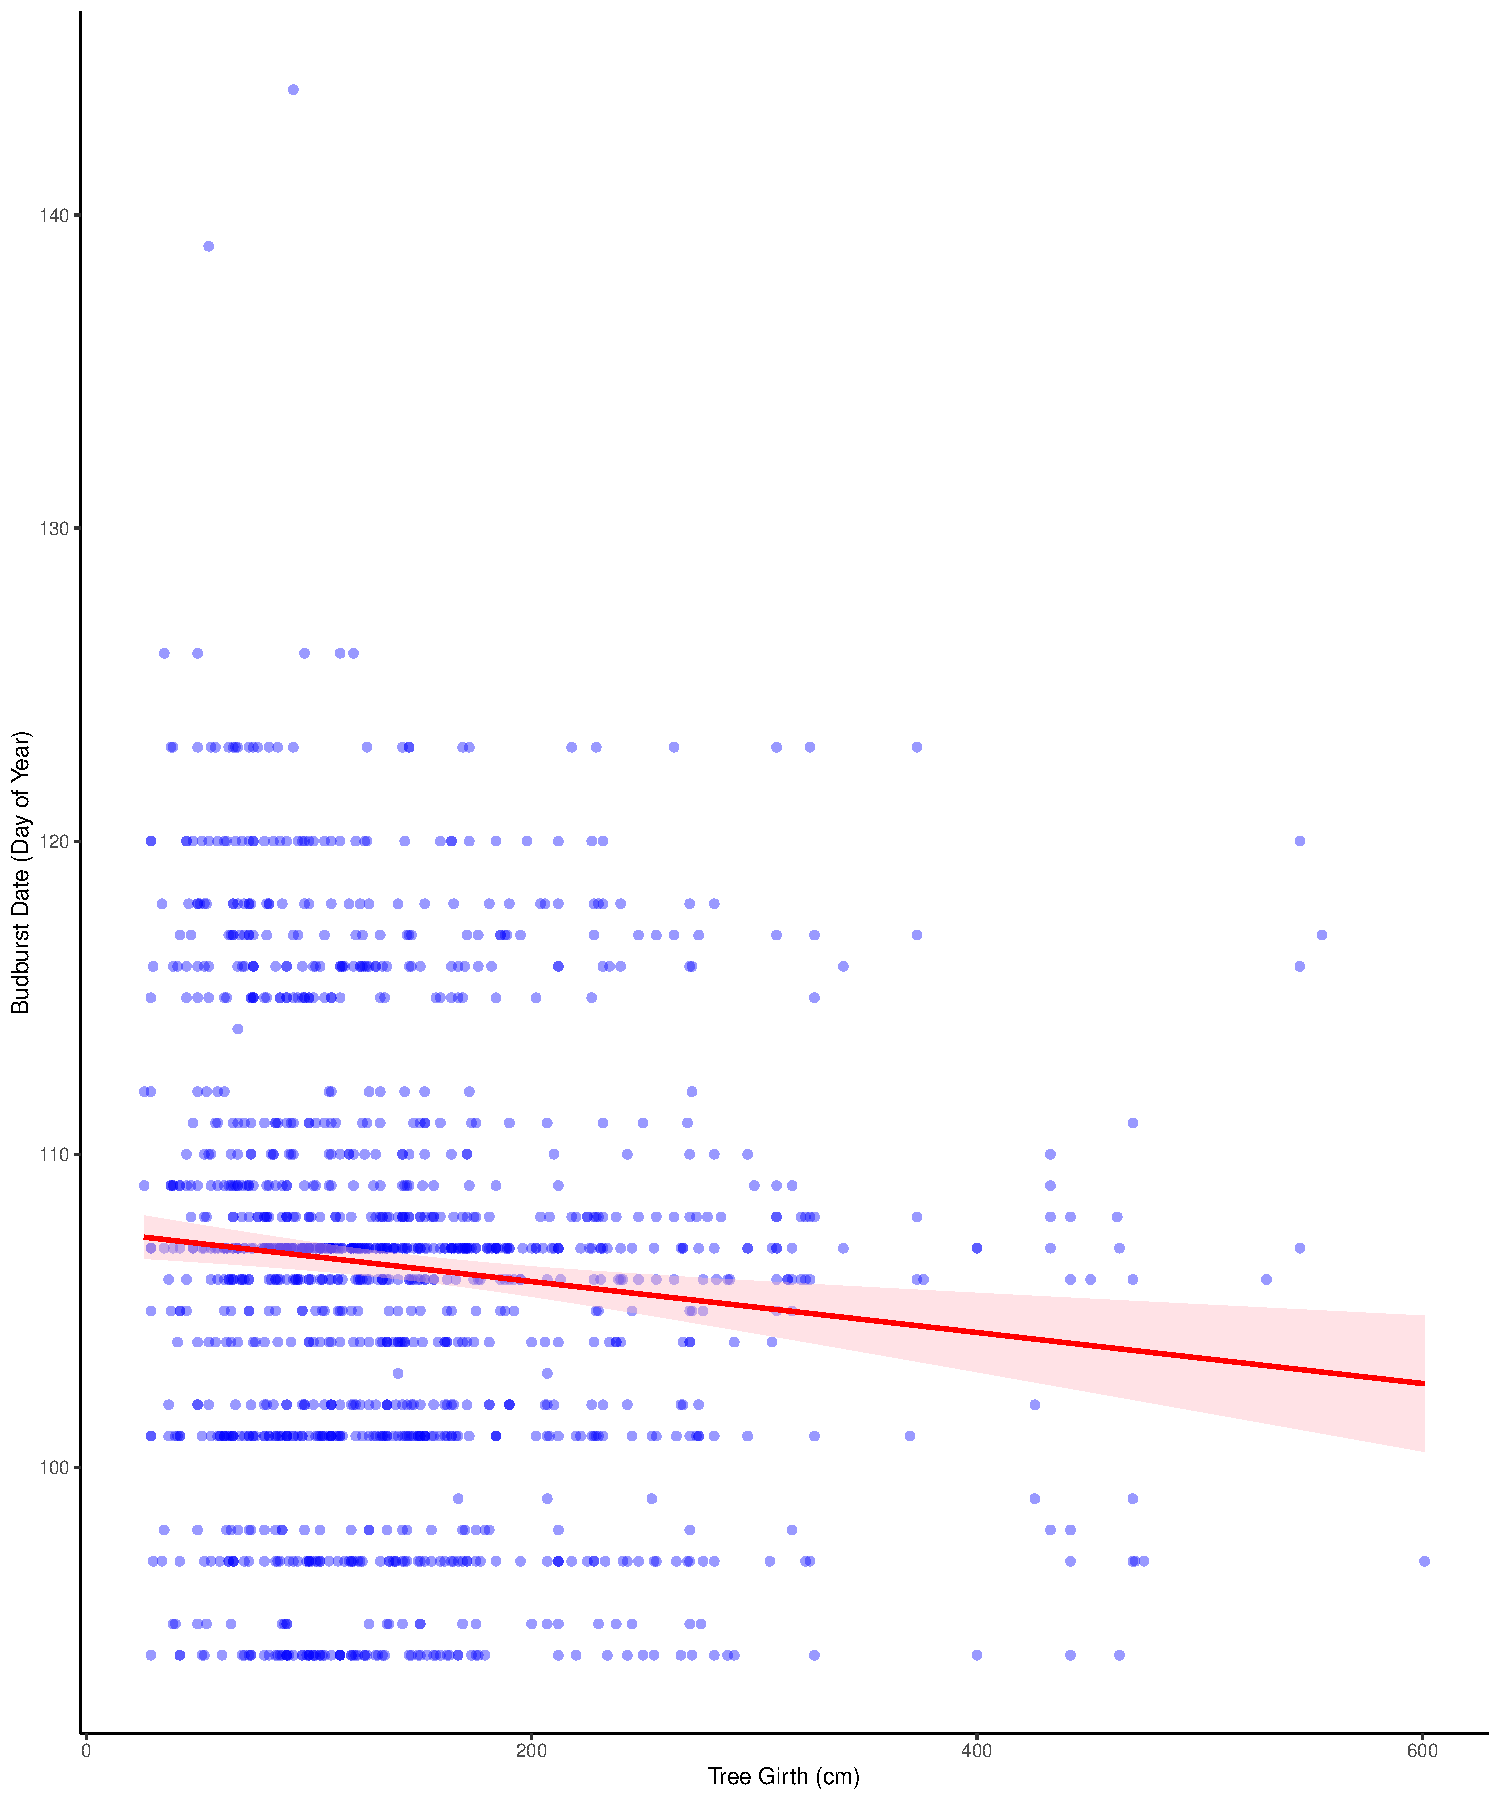
\includegraphics[width=0.8\textwidth]{../results/Plot.pdf}  % Adjust width as needed
        \caption{Relationship between budburst date and tree girth. Each point represents a budburst observation. Regression line with 95\% confidence interval is plotted based on the linear model coefficients in Table 1.}
        \label{fig:pdfimage}
    \end{figure}

\end{document}
